\documentclass[man,a4paper,noextraspace]{apa6}\usepackage[]{graphicx}\usepackage[]{color}
%% maxwidth is the original width if it is less than linewidth
%% otherwise use linewidth (to make sure the graphics do not exceed the margin)
\makeatletter
\def\maxwidth{ %
  \ifdim\Gin@nat@width>\linewidth
    \linewidth
  \else
    \Gin@nat@width
  \fi
}
\makeatother

\definecolor{fgcolor}{rgb}{0.345, 0.345, 0.345}
\newcommand{\hlnum}[1]{\textcolor[rgb]{0.686,0.059,0.569}{#1}}%
\newcommand{\hlstr}[1]{\textcolor[rgb]{0.192,0.494,0.8}{#1}}%
\newcommand{\hlcom}[1]{\textcolor[rgb]{0.678,0.584,0.686}{\textit{#1}}}%
\newcommand{\hlopt}[1]{\textcolor[rgb]{0,0,0}{#1}}%
\newcommand{\hlstd}[1]{\textcolor[rgb]{0.345,0.345,0.345}{#1}}%
\newcommand{\hlkwa}[1]{\textcolor[rgb]{0.161,0.373,0.58}{\textbf{#1}}}%
\newcommand{\hlkwb}[1]{\textcolor[rgb]{0.69,0.353,0.396}{#1}}%
\newcommand{\hlkwc}[1]{\textcolor[rgb]{0.333,0.667,0.333}{#1}}%
\newcommand{\hlkwd}[1]{\textcolor[rgb]{0.737,0.353,0.396}{\textbf{#1}}}%

\usepackage{framed}
\makeatletter
\newenvironment{kframe}{%
 \def\at@end@of@kframe{}%
 \ifinner\ifhmode%
  \def\at@end@of@kframe{\end{minipage}}%
  \begin{minipage}{\columnwidth}%
 \fi\fi%
 \def\FrameCommand##1{\hskip\@totalleftmargin \hskip-\fboxsep
 \colorbox{shadecolor}{##1}\hskip-\fboxsep
     % There is no \\@totalrightmargin, so:
     \hskip-\linewidth \hskip-\@totalleftmargin \hskip\columnwidth}%
 \MakeFramed {\advance\hsize-\width
   \@totalleftmargin\z@ \linewidth\hsize
   \@setminipage}}%
 {\par\unskip\endMakeFramed%
 \at@end@of@kframe}
\makeatother

\definecolor{shadecolor}{rgb}{.97, .97, .97}
\definecolor{messagecolor}{rgb}{0, 0, 0}
\definecolor{warningcolor}{rgb}{1, 0, 1}
\definecolor{errorcolor}{rgb}{1, 0, 0}
\newenvironment{knitrout}{}{} % an empty environment to be redefined in TeX

\usepackage{alltt}

\title{Always Use the Separate Variances t Test for Two Independent Groups}
\shorttitle{Separate Variances t Test}
\author{Joshua D. Wondra and Richard Gonzalez}
\affiliation{University of Michigan}

\abstract{This is an abstract}
\keywords{t test, new statistics}
\IfFileExists{upquote.sty}{\usepackage{upquote}}{}
\begin{document}
\maketitle

    Data analysis involves a series of decisions on the part of the researcher about which test best answers the research question, whether the data fit the requirements of the test, and whether there are alternative options that will do a better job. Recent discussions of false positives in psychology research (CITATIONS) highlight the tension between two valued outcomes of the decision process. On the one hand, researchers want to avoid mistakenly claiming that there is a true effect where none exists, or avoid false positives. On the other hand, researchers want to find true effects where they do exist, which involves concerns about power. In addition to concerns about rejecting the null hypothesis and concluding that there is an effect, there is the concern with accurate effect size estimation (CITATIONS). Because so many studies are underpowered, those that exist in published research must be false positives or high estimates of the true effect size, or so the argument goes (CITATIONS).

    One of the first decisions that most researchers learn to do with their data is to compare the means of two groups to determine whether they differ from each other--they run a t test. But even this simple test presents a choice between the classic Student's t test (CITATION) or the alternative Welch-Satterthwaite test (CITATION). We were interested in how researchers can best make decisions between these tests that balance the concerns between false positives, power, and effect size estimation. 

    Most researchers learn about Student's t test in the first statistics class that they ever take. When using Student's t test to compare independent group means, you make three assumptions. 
    
    1. Normality: The population for each group has a normal distribution.

    2. Independence: All observations are independent of each other, meaning that the probability of one observation having a particular value does not depend on the probability of another observation having a particular value.

    3. Equal variances: The population variances for the two groups are equal. 

If either the data or the study design suggests that one or more of the assumptions have been violated, then Student's t test is an inappropriate choice to compare the means. 

    You are more likely to reject the null hypothesis and conclude that there is a difference in the group means as the value of the t test or the degrees of freedom get larger. The value of the test is a parameter estimate divided by the standard error of that estimate. When the test is used to compare the means of two independent groups, it is the difference in group means divided by the standard error of that estimate. 
    
This means that you are more likely to reject the null hypothesis when the difference in means is large and the standard error is small. With the equal variances assumption, the estimate of the standard error of the difference in group means is based on a common variance that pools the estimates of the two group standard errors. The degrees of freedom are equal to the sum of the sample sizes of each group after subtracting one from each group, meaning that you are more likely to reject the null hypothesis as the sample sizes grow larger.

    Many researchers might not learn about the Welch-Satterthwaite test (hereafter called the Welch t test for the sake of brevity) in their formal statistical training, though most have encountered it in their own analysis. Researchers who use SPSS (CITATION) to analyze their data encounter the Welch test in the "Equal variances not assumed" line that appears by default whenever they run a t test. Researchers who use \texttt{R} (CITATION) get the Welch test results by default when they use the \texttt{t.test()} function and can only get the Student's t test results by setting the \texttt{var.equal} argument to \texttt{TRUE}.
    
        As with Student's t test, the Welch t test assumes normality and independence; however, it does not assume that the population variances are equal. As a result, the standard error of the difference in means is based on separate group variances instead of a common variance. Additionally, the Welch t test decreases the degrees of freedom to the extent that the group variances differ, though the degrees of freedom will be identical to the Student's t test when variances are equal. Because of these differences, the two tests can disagree about whether there is a difference in group means. The Welch penalty to the degrees of freedom pushes the Welch test in the direction of being more conservative and less likely to reject the null. On the one hand, this might lead to more correct decisions if the equal variances violation leads the Student's t test to have an inflated false positive rate. On the other hand, which might concern researchers that the Welch test has too little power to detect real effects. 
        
    However, the Welch test is not necessarily always more conservative. The power of the t test to detect effects also depends on the standard error of the test, and as a result the Welch test could be more powerful under conditions when the separate variances standard error is smaller than the pooled variances standard error of Student's test. Notably, the pooled and separate variance standard errors are equal to each other when either the sample sizes or the variances of the two groups are identical, so the Welch test will only be more powerful when both the variance and sample sizes are unequal.  
    
    How do we decide which test to use? The typical approach is to use Student's t test unless there is evidence that the populations have unequal variances. The challenge is how to decide that there is sufficient evidence of unequal population variances. One option is to run another test of the null hypothesis that the variances are equal, such as Levene's test for homogeneity, which shows up by default in SPSS, and use the Welch test if you reject the null. This is usually seen as an ineffective strategy because tests of assumptions make their own assumptions that go unchecked and they are sensitive to sample size (CITATIONS). A second option is to visualize the data using boxplots and make a visual judgment about whether the variances appear to differ. With smaller sample sizes, one can tolerate larger apparent differences in variances. This strategy can be enhanced by simulating data for two groups of sample sizes equal to your own data, changing whether the variances are equal or unequal, and seeing how variable the boxplots look under each condition. A third option that has not been tested to our knowledge is to examine the ratio of the degrees of freedom between the classic and Welch test. If the two differ to a large extent, then it might be a sign that the group variances differ. We examine this strategy in our simulations. A fourth option is to change that starting mentality – when variances and sample sizes are equal, the Welch test is equivalent to Student's t test. If it using the Welch test generally lead to better decisions than Student's t test under both these ideal and non-ideal conditions, then instead of using Student's t test by default it might be better to always use the Welch test.
    
    We examined these possibilities in a Monte Carlo simulation study and examined the false positives, power, and coverage probability of Student's and Welch's t tests under different conditions. 

\section{Method}
    We ran Monte Carlo simulations of two independent groups with normally distributed data. We examined the type I error rate, power, and coverage probability for both the equal variances t test and the separate variances t test under different conditions. We varied the variance ratio ($\sigma_{1}/\sigma_{2}$ = 1/5, 1/2, 1, 2, or 5), sample size ratio ($n_{1}/n_{2}$ = 1, 2/3, or 1/2), and sample sizes (small $n$ = 20, 50, or 100). 
    
    Additionally, we varied the size of the difference in group means using Cohen’s d values of 0, .2, .5, and .8. Importantly, Cohen’s d requires the group variances to be equal because it uses a pooled variance. For the conditions with unequal variances, we computed the mean differences for the same Cohen’s d values as though the two different population variances were incorrect estimates of a common population variance. This is comparable to the implicit assumption that researchers make when they use the equal variances t test on data that violate the equal variances assumption.
    
    The full set of conditions is displayed in Table 1. For each condition, we set the seed to 2184 and ran 10,000 simulations. We did not simulate the conditions with equal sample sizes and variance ratios of 2 and 5 because they were identical to the conditions with equal sample sizes and variance ratios of ½ and 1/5. 

\section{Results}    

\subsection{Boxplots} One option for deciding whether the group variances are equal is to examine boxplots. Figure 1 displays boxplots for the first simulation each condition when sample sizes are equal. When variances are unequal, the larger variance is for the group to the right. When the sample sizes are smaller, it can be more difficult to tell whether the variances are unequal or not. When the sample sizes are 20, the variance of one group looks a bit larger than the other when they are really equal and the variances look approximately equal when one group has twice the variance of the other. As the sample size and increases, it becomes clearer to see whether there is a violation - at 100 subjects per condition, when variances are equal the boxes and whiskers are approximately the same length, and when variances are unequal both the box and whiskers appear wider in the group with the bigger variance. By examining several additional simulations it would be possible to see how much variability in the boxplots is normal when variances are equal or unequal.
   
\begin{knitrout}
\definecolor{shadecolor}{rgb}{0.969, 0.969, 0.969}\color{fgcolor}
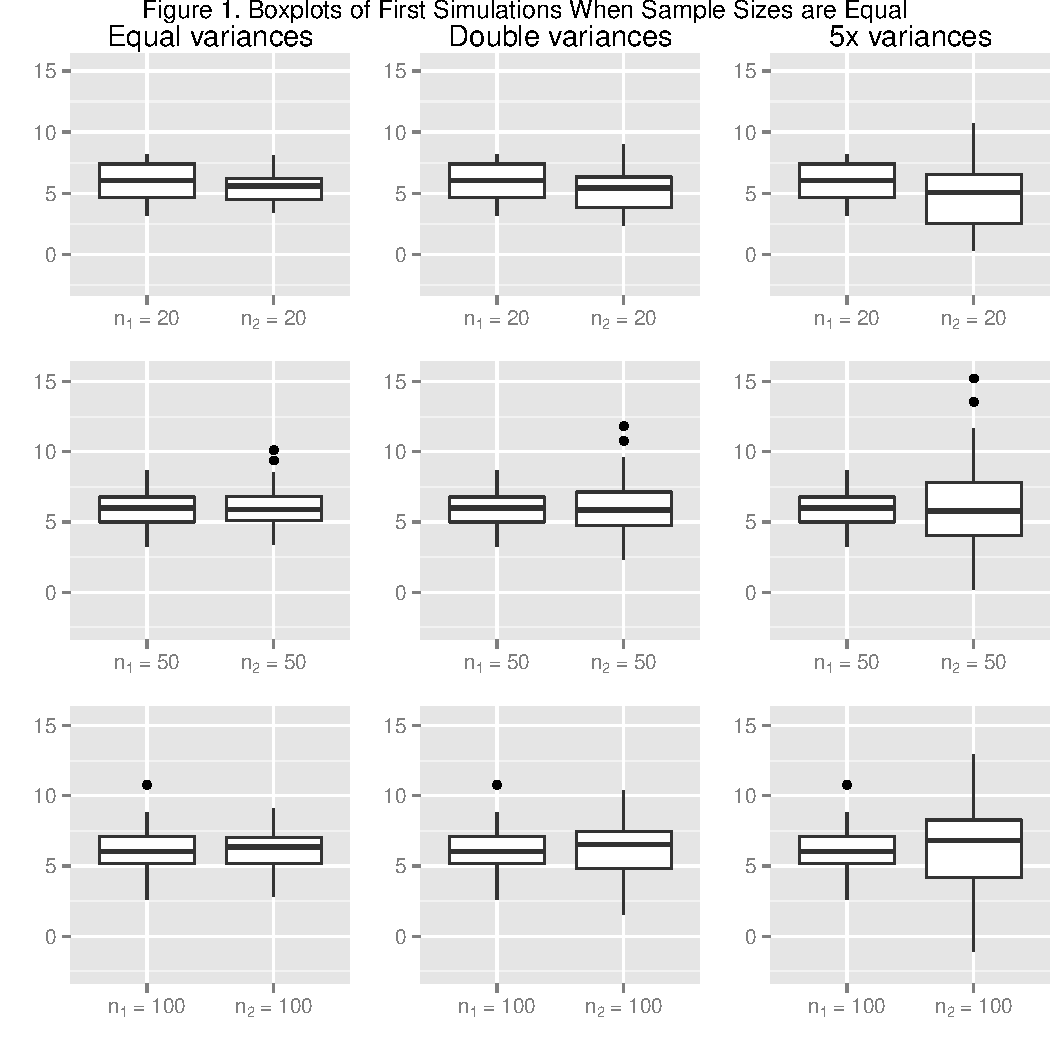
\includegraphics[width=\maxwidth]{figure/equalNboxplots} 

\end{knitrout}

Figure 2 displays a sample of boxplots for simulations when the sample size ratio and variance ratio are both changing (NOTE: I'm not sure that this adds much so we might just drop it).

\begin{knitrout}
\definecolor{shadecolor}{rgb}{0.969, 0.969, 0.969}\color{fgcolor}
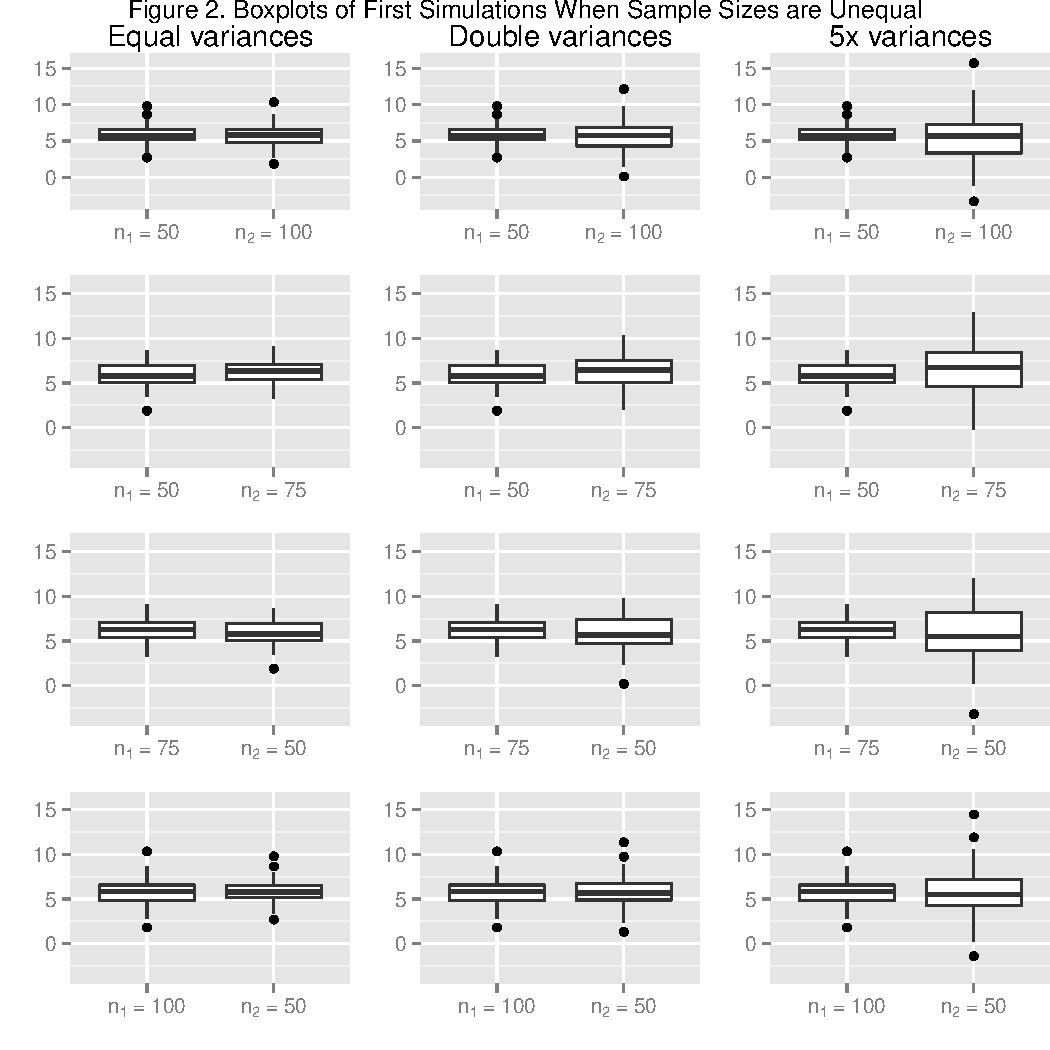
\includegraphics[width=\maxwidth]{figure/differentNboxplots} 

\end{knitrout}

\subsection{Does the df Ratio Help?}
    We examined whether looking at ratio of the Welch degrees of freedom to the classic t test degrees of freedom would provide a heuristic for deciding that equal variances does not hold. Figure 3 displays boxplots of the ratio of Welch degrees of freedom to the classic t test degrees of freedom as sample sizes increase when  the variance and sample size ratios equal. As the sample sizes increase, the degrees of freedom ratio stays close to 1. 

\begin{knitrout}
\definecolor{shadecolor}{rgb}{0.969, 0.969, 0.969}\color{fgcolor}
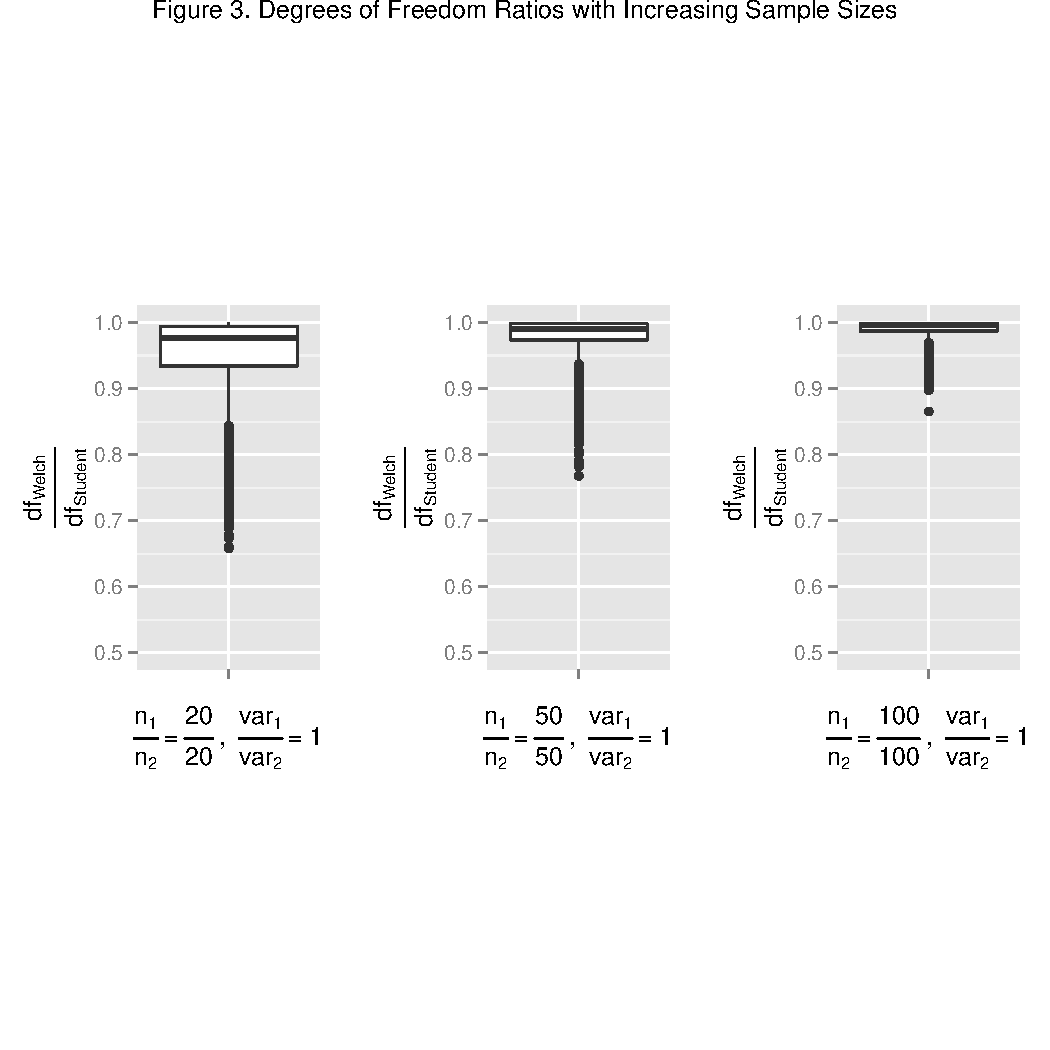
\includegraphics[width=\maxwidth]{figure/dfratiosNincrease} 

\end{knitrout}

    Figure 4 displays the ratio as the group variances become increasingly different when both the sample size and the sample size ratio stay the same. Under this condition, the distribution moves away from 1 as the difference in group variances increases.

\begin{knitrout}
\definecolor{shadecolor}{rgb}{0.969, 0.969, 0.969}\color{fgcolor}
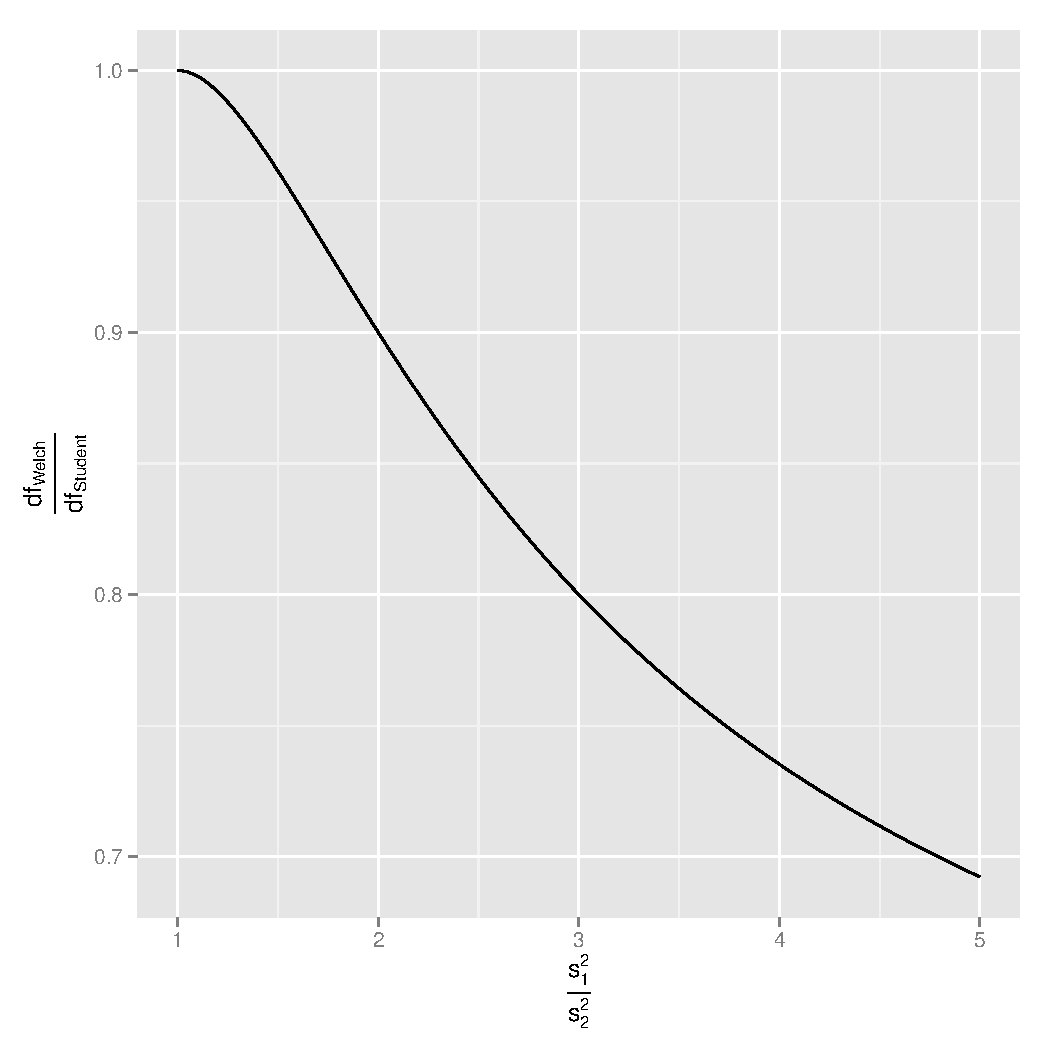
\includegraphics[width=\maxwidth]{figure/dfratiosDiffvars} 

\end{knitrout}

    In the first two plots, the degrees of freedom ratios are generally above 95\% when variances are equal and below 95\% when they differ. A useful heuristic might be to assume unequal variances when the ratio falls below 95\%. But now look what happens when the variances are equal and the sample size ratio changes in Figure 5. Here too the ratio drops when the sample sizes become increasingly uneven, even though the variances stay the same. Our 95\% heuristic would lead us astray and we would incorrectly conclude that the variances are unequal.

\begin{knitrout}
\definecolor{shadecolor}{rgb}{0.969, 0.969, 0.969}\color{fgcolor}
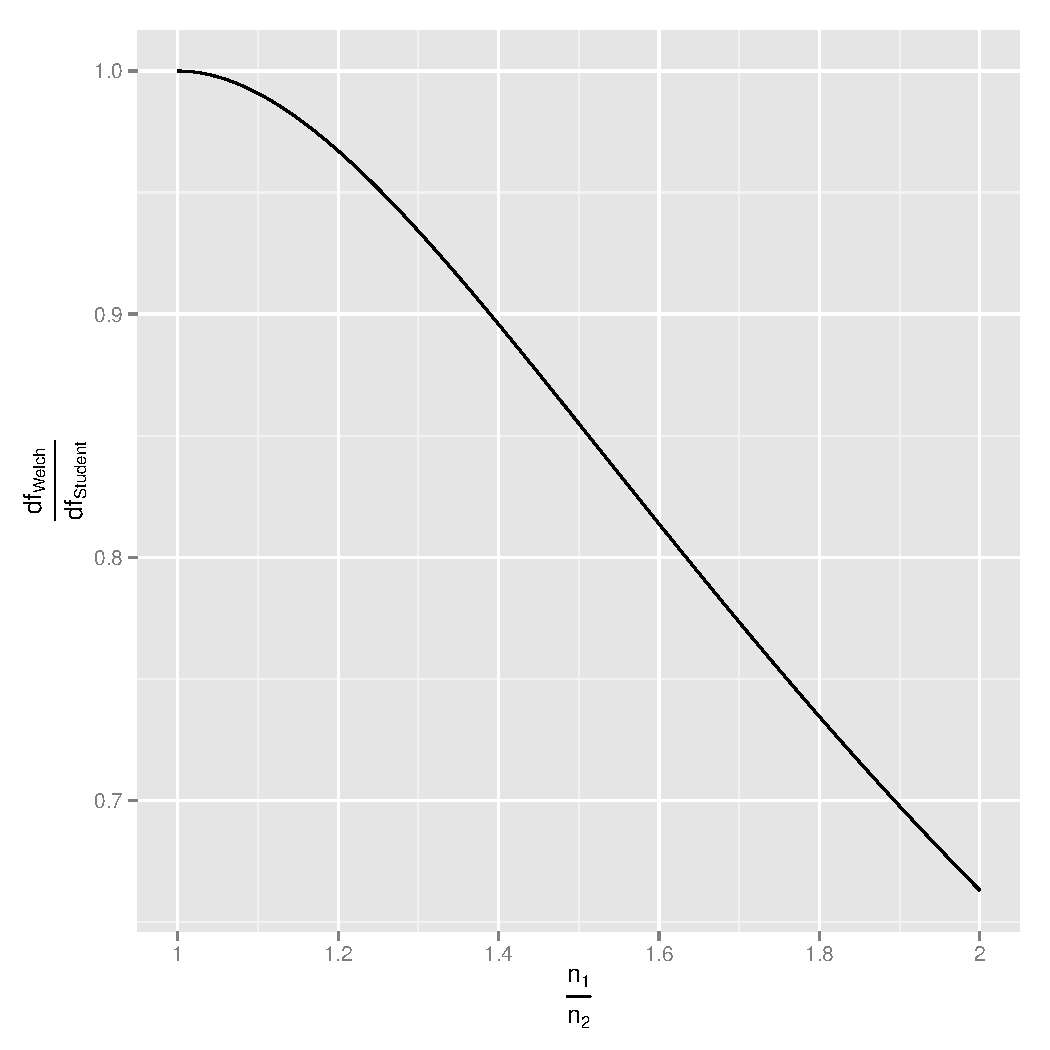
\includegraphics[width=\maxwidth]{figure/dfratiosDiffNratios} 

\end{knitrout}

    Finally, Figure 6 demonstrates one example of what happens to the degrees of freedom ratio when the variances become increasingly unequal and the sample sizes are unequal. In this case, the effect of different variances depends on whether the larger group has the larger variance or the smaller variance. In the first row, when the larger group has the larger variance, the move from equal to unequal variances actual counteracts the effect of the unequal sample sizes, and the degrees of freedom are generally higher at both unequal variance ratios that we sampled. However, in the second row, when the larger group has the smaller variance, the degrees of freedom ratio drops as the variances become increasingly unequal. 

\begin{knitrout}
\definecolor{shadecolor}{rgb}{0.969, 0.969, 0.969}\color{fgcolor}
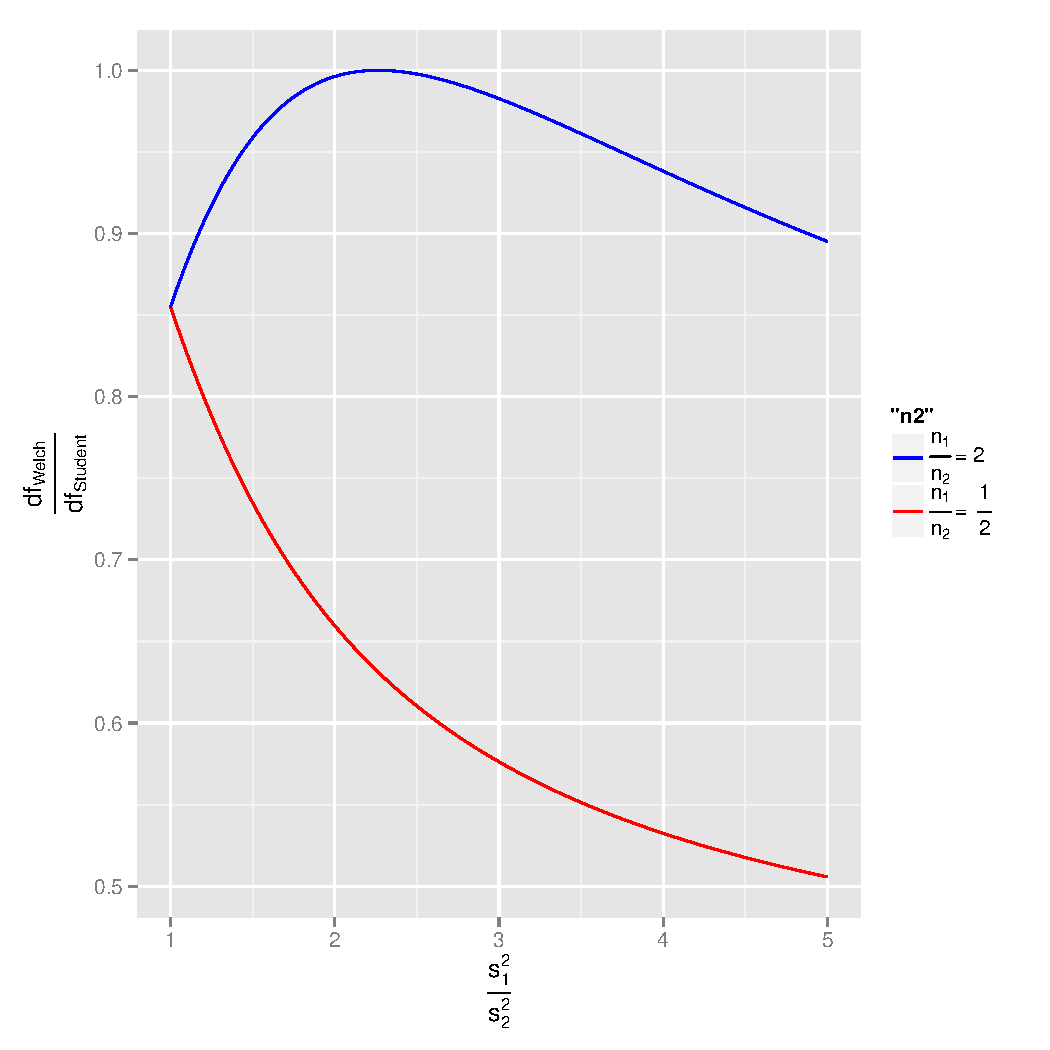
\includegraphics[width=\maxwidth]{figure/dfratiosDiffvarsDiffNratios} 

\end{knitrout}

    In short, the usefulness of a heuristic based on the ratio of degrees of freedom from the Welch test to degrees of freedom from Student's test is limited to cases when the sample sizes are equal. 

    One of the concerns about using the Welch test as an alternative to Student's t test is that the penalty on the degrees of freedom makes it difficult to find effects. The boxplots show that under ideal conditions, when the true population variances and the sample sizes are equal, the penalty is small. Even under non-ideal conditions, when both the population variances and the sample sizes are unequal, there is variability in the penalty depending on the specific configuration of sample sizes and variances.

\subsection{When Does Each Test Perform Best?}
    The simple rule based on the degrees of freedom penalty did not work well, so we decided to examine when the Welch and Student t tests would perform best based on the sample size, variance ratio, and sample size ratio. We examined how well each test balances the concerns about false positives, power, and estimation, and we report the observed Type I error rates, observed power, and coverage probability for the classic and separate variance t tests over the 10000 simulations.
\subsection{Type I Error Rates}


    In this section we report type I error rates for the classic and separate variance t tests when the null hypothesis is true. Prior research has demonstrated that when either sample sizes or variances are equal, the type I error rates are preserved at .05 for both tests (CITATIONS). This prior work has typically examined sample sizes that are far smaller than the typical psychology experiment.
    
    Figure 7 displays the type I error rate for the classic t test across the different conditions. Consistent with prior research, the type I error rate remained close to .05 when either the sample size or the population variances were equal, but it varied widely when both population variances and sample sizes were unequal. On the left side of Figure 1, when the group with the larger sample size had the larger variance, the type I error rate dropped as low as about .01, whereas on the right side, when the group with the larger sample size had the smaller variance, the type I error rate rose as high as .12, which is more than double the normally accepted false positive rate. 
    
\begin{knitrout}
\definecolor{shadecolor}{rgb}{0.969, 0.969, 0.969}\color{fgcolor}
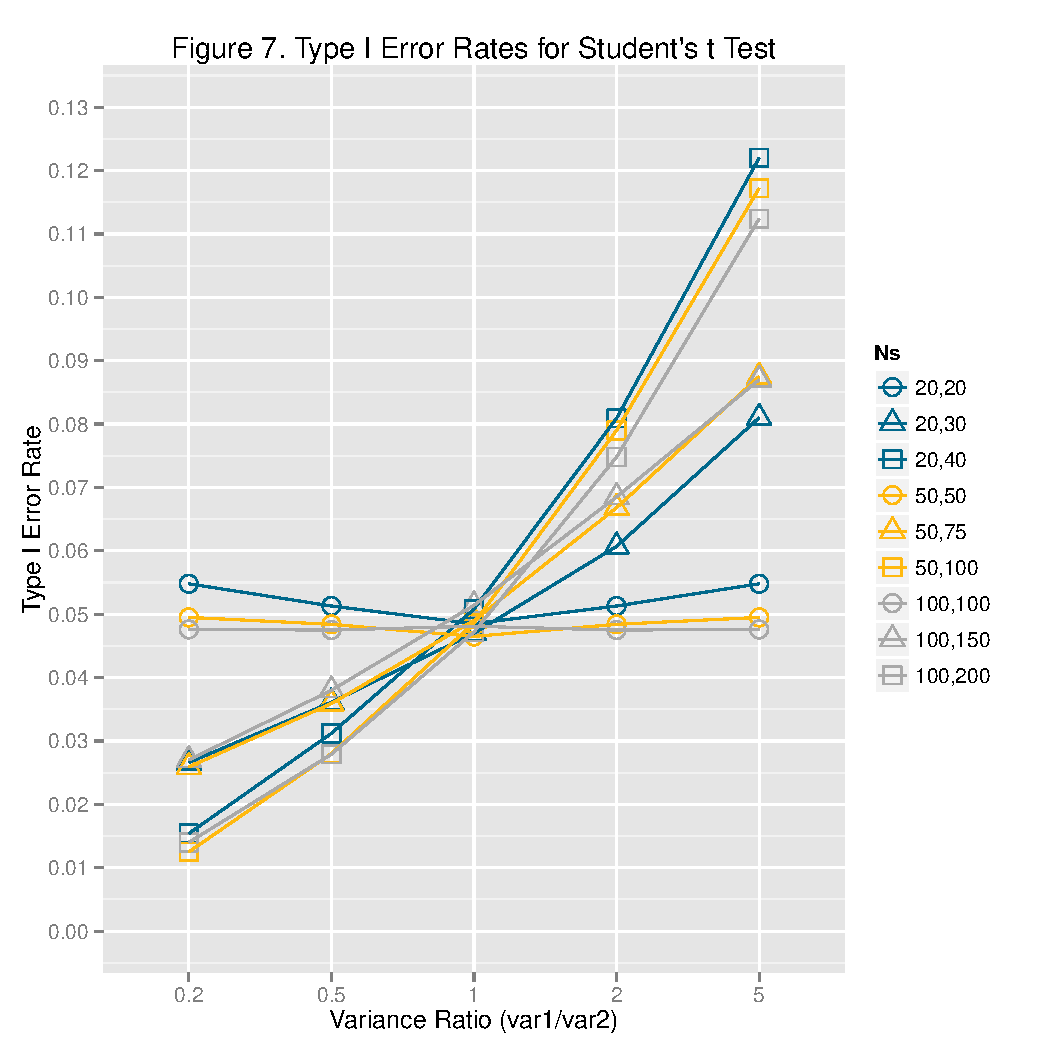
\includegraphics[width=\maxwidth]{figure/type1_classic_plot} 

\end{knitrout}

    Figure 8 displays the type I error rate for the separate variance t test across the different conditions. In contrast to the classic t test, and consistent with prior research, the type I error rate remained close to .05 across all conditions. 
    
    Here we see the degrees of freedom penalty at work. Our boxplots showed that the penalty was greatest when the large group had the small variance, which reduced the false positive rate of the classic t test. In contrast, the penalty was less severe when the large group had the large variance, so that the Welch test did not reduce the type I error rate beyond the .05 level. Additionally, we can see the different effects of using pooled and separate variances to compute the standard errors. Because the pooled variance of the classic t test weighs the larger sample more heavily, it becomes more liberal when the associated variance is small and more conservative when the associated variance is large. 

\begin{knitrout}
\definecolor{shadecolor}{rgb}{0.969, 0.969, 0.969}\color{fgcolor}
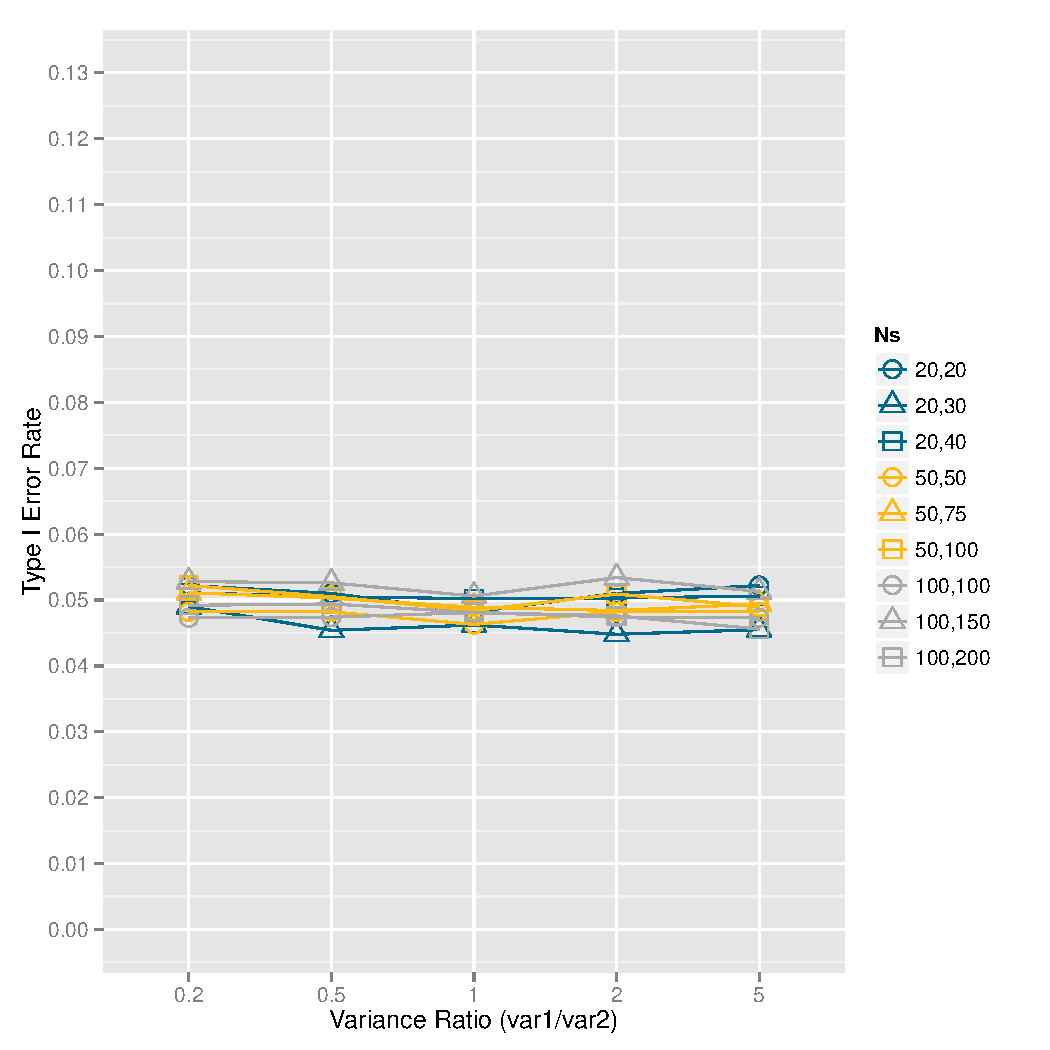
\includegraphics[width=\maxwidth]{figure/type1_Welch_plot} 

\end{knitrout}

\subsection{Power}




    Figure 9 displays the power of the classic and Welch tests to detect small, medium, and large effects under the different conditions. Overall, the classic t test is more powerful when the large sample has the smaller variance, whereas the Welch test is more powerful when the small sample has the smaller variance. These differences are the most dramatic when one sample is twice the size of the other. 
    
    The conditions in which the classic t test has the greatest power over the Welch test, when one sample is twice the size of the other and the large sample has the small variance, are the same conditions in which the classic t test had a risk of doubling the false positive rate. In contrast, the Welch test was more powerful than the classic test under other conditions and never inflated the type I error rate.

    Taken together, the type I error rates and power favor the Welch test over the classic t test as better balancing researcher concerns.

\begin{knitrout}
\definecolor{shadecolor}{rgb}{0.969, 0.969, 0.969}\color{fgcolor}
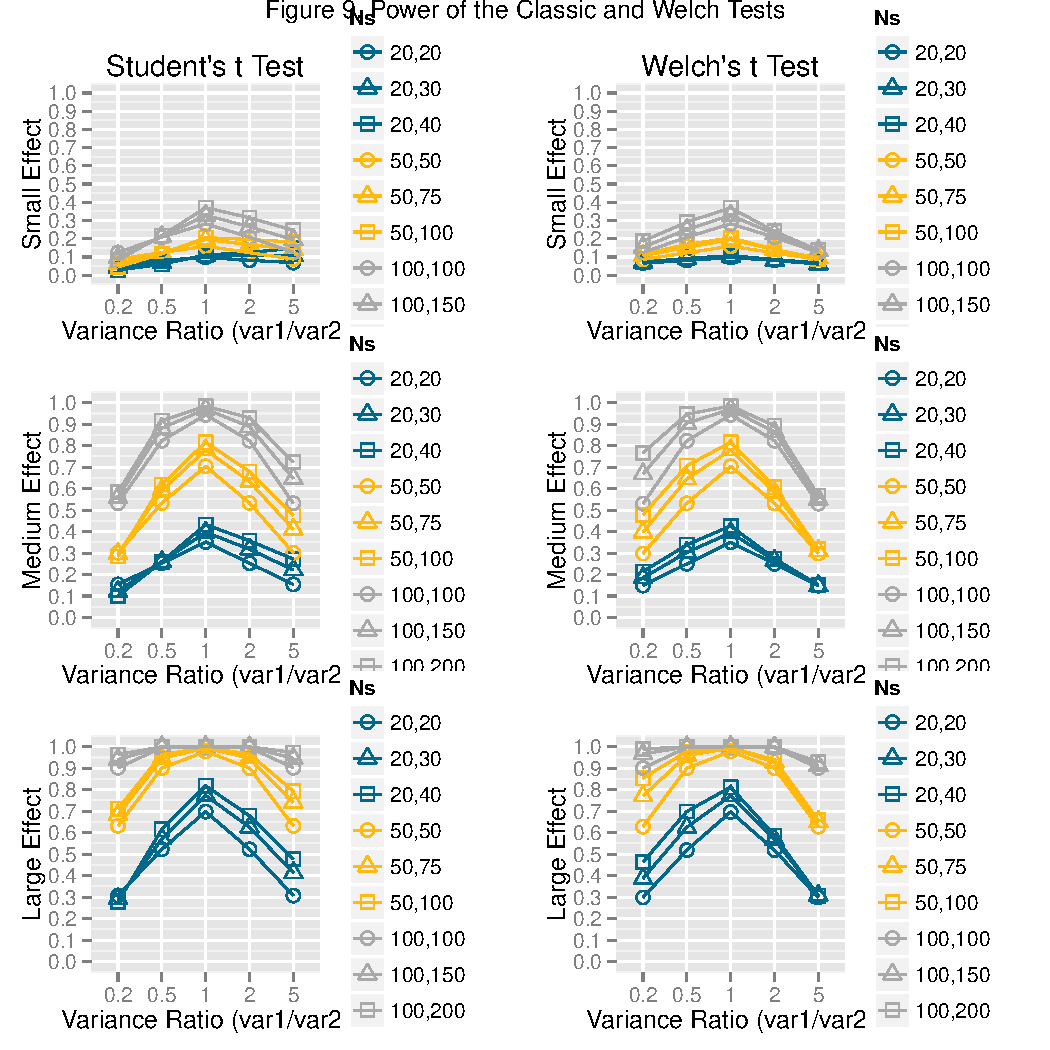
\includegraphics[width=\maxwidth]{figure/plot_power} 

\end{knitrout}

\subsection{Coverage Probability}
Because the accuracy of a confidence interval is influenced by the variance and sample size, but not by the true effect size, we only show the coverage probability when the null hypothesis is true (the coverage probabilities are identical across all effect sizes). Table 10 displays the coverage probability, which is how often the 95\% confidence interval contains the true mean difference in groups, for the two tests under the different conditions. The coverage probability for the classic t test varies dramatically. When it is the least powerful, it is the most accurate. When it is the most powerful, the effect size estimation is the least accurate, and what seems to be a 95\% confidence interval drops as low as an 88\% confidence interval. Once again, the Welch test retains the expected 95\% rate and turns out to best meet a researcher's concerns. 






\begin{knitrout}
\definecolor{shadecolor}{rgb}{0.969, 0.969, 0.969}\color{fgcolor}\begin{kframe}


{\ttfamily\noindent\color{warningcolor}{\#\# Warning: Removed 3 rows containing missing values (geom\_point).}}\end{kframe}
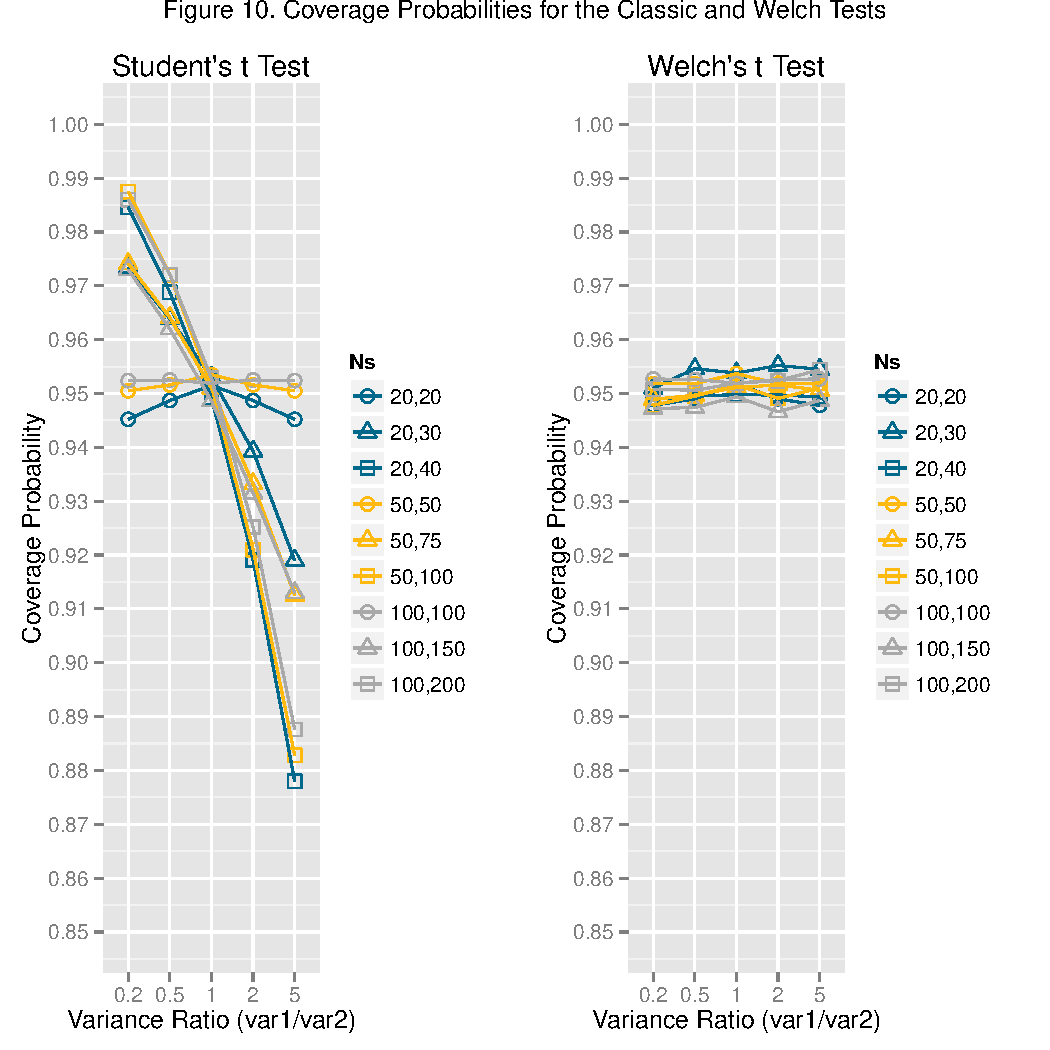
\includegraphics[width=\maxwidth]{figure/coverage_plots} 

\end{knitrout}


\section{Discussion}
    Make a note that our df ratio rule works best when it doesn't matter - when sample sizes are equal.
    
    In much experimental work, the choice between the tests is probably fine if the experimenter ensures that sample sizes are equal. This is generally not an option with pre-existing groups. 



\end{document}
